\chapter{Estado del arte}
\label{chapter:arte}

En este capítulo se presentan los conceptos básicos de las redes neuronales convolucionales, así como los trabajos más relevantes en el campo de la detección de polinizadores a partir de imágenes utilizando este tipo de redes. Luego de esto, se expone lo referente al preprocesamiento de las imágenes. Posteriormente, se resume una metodología para realizar la reconstrucción de redes de polinización a partir de datos observacionales. Estas son las técnicas fundamentales que se van a usar en lo largo del proyecto.

\section{Reconocimiento de imágenes}

Se entiende por «reconocimiento de imágenes» a la tarea de identificar y localizar objetos en una imagen. Esta tarea se puede dividir en dos sub-tareas: clasificación y detección. La clasificación consiste en identificar el objeto en la imagen, mientras que la detección consiste en identificar su ubicación en la imagen (\textit{bounding box}). Para el caso de la clasificación, se tiene como entrada una imagen y se obtiene como salida una etiqueta que identifica el objeto en la imagen. Estas etiquetas pertenecen a un conjunto finito de categorías preestablecidas.

\section{Origen de las redes neuronales convolucionales}

Las redes neuronales convolucionales (CNN por sus siglas en ingles \textit{Convolutional Neural Network}) son un tipo de red neuronal artificial que se utiliza principalmente para el procesamiento de imágenes. Las CNN se inspiran en la corteza visual de los animales, específicamente en el sistema visual primario de los gatos, descrito por Hubel y Wiesel en 1962 \cite{hubel-1962}. En este sistema, las neuronas individuales responden a estímulos en regiones restringidas del campo visual conocidas como campos receptivos. Estas neuronas se organizan en capas, donde cada capa se compone de un conjunto de neuronas que responden a un campo receptivo específico. Las neuronas de la primera capa responden a estímulos simples, como líneas y bordes, mientras que las neuronas de capas posteriores responden a estímulos más complejos, como formas y objetos. Las neuronas de capas posteriores se activan cuando se activan las neuronas de capas anteriores, lo que permite la detección de características cada vez más complejas. Este proceso se conoce como extracción de características.

El inicio de las CNN se remonta a 1982, cuando Fukushima propuso la arquitectura Neocognitron \cite{fukushima-1982}, en la cual se presentaban células simples y complejas que sería el análogo a lo que actualmente se conoce como las capas de una CNN. No fue hasta 1989 cuando LeCun et al. \cite{lecun-1989} propusieron la arquitectura LeNet-5, que se considera la primera CNN moderna. Desde entonces, las CNN han sido ampliamente utilizadas en el campo del procesamiento de imágenes y en el reconocimiento de objetos.

El inicio de las CNN se remonta a 1982, cuando Fukushima propuso la arquitectura Neocognitron \cite{fukushima-1982}, sentando las bases para lo que más tarde serían las capas de una CNN. La evolución continuó en 1989 con LeCun et al. \cite{lecun-1989} y la introducción de la arquitectura LeNet-5, considerada la primera CNN moderna. Sin embargo, el verdadero salto hacia el Aprendizaje Profundo (\textit{Deep Learning}) se produjo en la última década, impulsado por varios factores clave.

El desarrollo de hardware más potente, especialmente GPUs, permitió el entrenamiento de redes neuronales más profundas y complejas \cite{alzubaidi-2021}. Paralelamente, avances en algoritmos y técnicas de entrenamiento, como la función de activación ReLU y la regularización mediante Dropout, optimizaron el proceso de aprendizaje para redes más profundas \cite{GU2018354}. La aparición de arquitecturas revolucionarias, como AlexNet en 2012 , demostró mejoras significativas en tareas de procesamiento de imágenes y reconocimiento de objetos \cite{russakovsky-2015}.


\subsection{Arquitectura y conjuntos de entrenamiento}

En la actualidad, existen varias arquitecturas que han dado buenos resultados en el campo del reconocimiento de objetos en imágenes. Algunas de estas son: AlexNet \cite{russakovsky-2015}, VGGNet \cite{simonyan2014very}, GoogLeNet \cite{7298594}, ResNet \cite{he2016deep}, entre otras. La mayoría de estas arquitecturas son entrenadas y evaluadas en el conjunto de datos ImageNet \cite{ImageNet}, que contiene más de 14 millones de imágenes. Este conjunto de datos brinda una amplia variedad objetos en las imágenes y, por lo tanto, se tienen resultados generales en lo que respecta al reconocimiento. Sin embargo, para lograr el reconocimiento de insectos, es necesario contar con conjuntos de datos más específicos y también arquitecturas enfocadas en este tipo de imágenes. 

En este trabajo, se han seleccionado las arquitecturas YOLOv5 y EfficientNet por su equilibrio único entre velocidad, precisión y eficiencia, esenciales para el análisis de grandes conjuntos de datos de imágenes de insectos. YOLOv5 sobresale en la detección rápida y precisa, vital para el análisis en tiempo real, y ha mostrado resultados prometedores en conjuntos de datos similares \cite{ahmad-2022}. Por su parte, EfficientNet destaca por su escalabilidad y alto rendimiento en la clasificación de imágenes, junto con un uso eficiente de recursos computacionales~\cite{bjerge-2023}, lo cual es crucial para la identificación precisa de especies en redes planta-polinizador. Esta combinación de características hace que ambas arquitecturas sean particularmente adecuadas para abordar los desafíos específicos del proyecto.

\subsection{YOLOv5}

YOLOv5 es una arquitectura de red neuronal convolucional para el reconocimiento de objetos en imágenes. Esta arquitectura se basa en la arquitectura YOLO (\textit{You Only Look Once}) \cite{redmon-2015}, la cual se caracteriza por ser un modelo de detección de objetos en tiempo real. El modelo toma como entradas las imágenes y produce como salida la detección de objetos, de manera específica: \textit{bounding box}, clase del objeto identificado, nivel de confianza.

De manera específica, la arquitectura de la red se detalla en \cite{nepal-2022} y se presenta el diseño de la misma en la Figura \ref{fig:yolov5}. En esta figura, se puede observar que la arquitectura se compone de una serie de bloques convolucionales denominada \textit{backbone}, la cual se encarga de realizar la detección de objetos en la imagen; aquí, \texttt{Conv} representa una capa convolucional, \texttt{C3} son tres capas convolucionales y un módulo en cascada con varios cuellos de botella y \texttt{SPP} es una capa de agrupación que se utiliza para que el modelo pueda identificar objetos de diferentes tamaños. Posteriormente, se tiene un grupo de capas denominado \textit{Neck}, la cual se encarga de realizar la fusión de características de las capas anteriores; en este grupo se tienen también capas \texttt{Upsample} (para aumentar el muestreo) y \texttt{Concat} (utilizada para cortar la capa anterior). Finalmente, se tiene un grupo de capas denominado \textit{Head}, el cual se encarga de realizar la detección de objetos en la imagen; en este grupo se tienen capas \texttt{Conv2d} (módulos de detección).

\begin{figure}[ht]
    \centering
    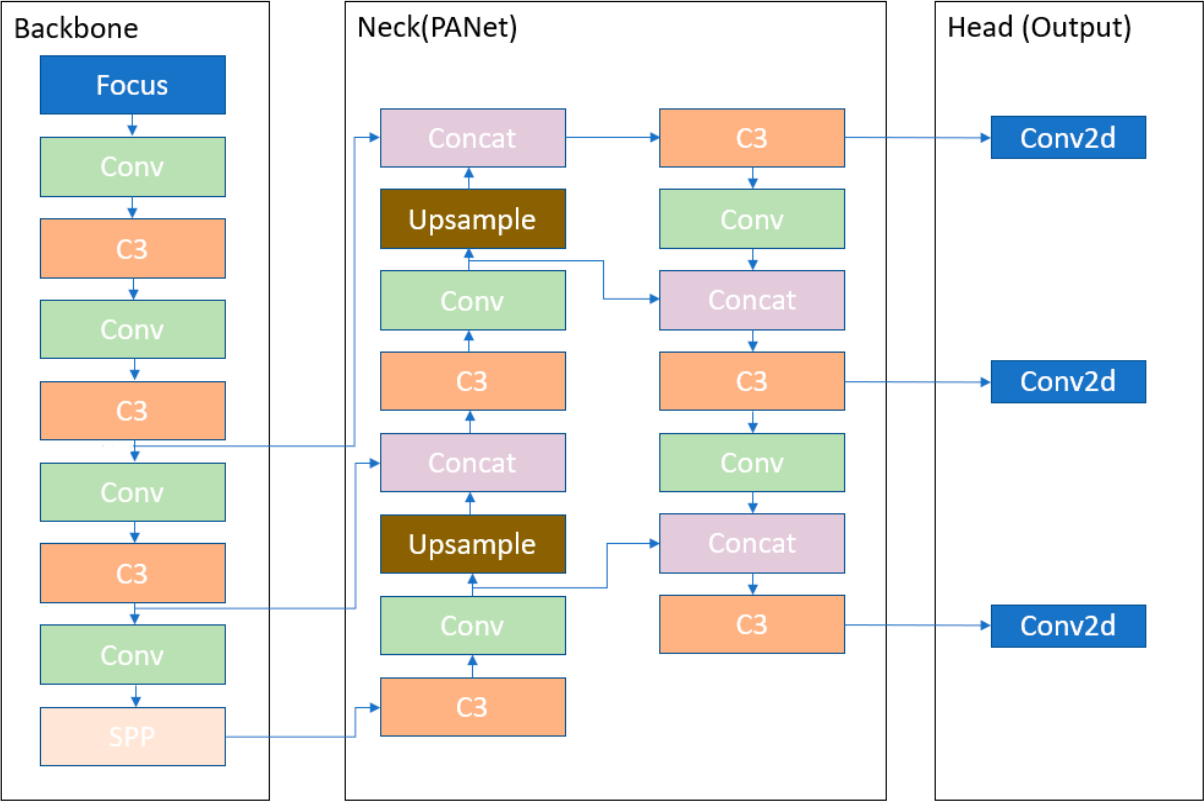
\includegraphics[width=0.95\textwidth]{Figuras/yolov5.png}
    \caption[Arquitectura de la red YOLOv5.]{Arquitectura de la red YOLOv5. Fuente: \cite{nepal-2022}.}
    \label{fig:yolov5}
\end{figure}


En \cite{nepal-2022} se indica que la arquitectura YOLOv5, al entrenarse sobre el conjunto de datos denominado DOTA (conjunto de imágenes aéreas), alcanza una precisión de 0.707 y un F1 Score de 0.655 en la tarea de reconocer y ubicar objetos en imágenes. En \cite{ahmad-2022}, se trabajó con esta arquitectura y se entrenó con un conjunto de datos de 7046 imágenes de insectos tomadas de internet (algunos ejemplos pueden verse en la Figura \ref{fig:yolov5-insects}). De igual manera, ser enfocó en la tarea de reconocer insectos en una imagen, en este caso, se obtuvo una precisión de entre el 0.7453 y el 0.9450 (con variaciones menores en la arquitectura); por el lado del F1 Score, se obtuvo entre 0.77 y 0.96. Por otro lado, en \cite{qi-2023}, se utilizó un conjunto de 25028 imágenes obtenidas por los autores del estudio; se obtuvo una precisión de 0.927 y un F1 Score de 0.932.

\begin{figure}[ht]
    \centering
    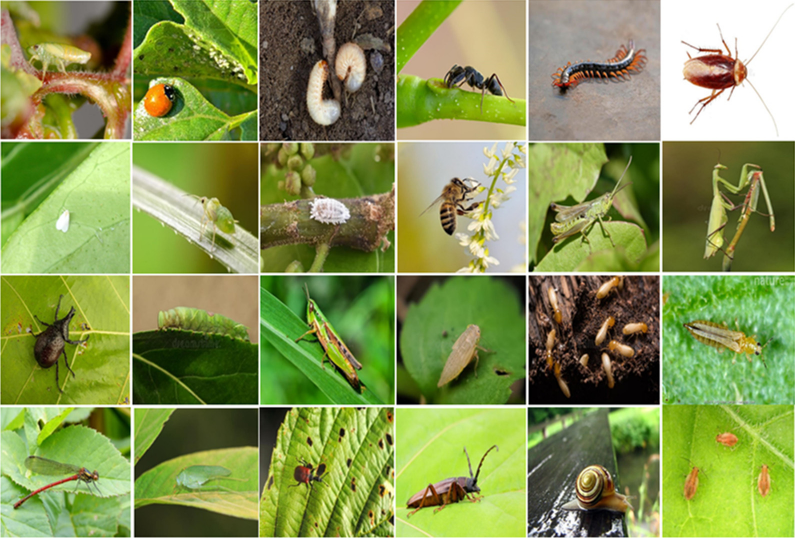
\includegraphics[width=0.95\textwidth]{Figuras/yolov5-insects.png}
    \caption[Ejemplos de imágenes de insectos utilizadas en {[6]}.]{Ejemplos de imágenes de insectos utilizadas en \cite{ahmad-2022}. Fuente: \cite{ahmad-2022}.}
    \label{fig:yolov5-insects}
\end{figure}

\subsection{EfficientNet}

EfficientNet \cite{tan-2019} es una arquitectura de red neuronal convolucional que se caracteriza por ser eficiente en términos de cómputo y parámetros. El modelo toma como entradas las imágenes y produce como salida la clasificación de objetos en la imagen, de manera específica: clase del objeto identificado y nivel de confianza. Cabe indicar que, a diferencia de YOLOv5, este modelo no realiza la localización del objeto.

En la Figura \ref{fig:efficientnet} se presenta la arquitectura de la red. Se aprecia que esta red tiene una estructura simple, pues es una capa convolucional (\texttt{Conv}), seguida de múltiples capas \texttt{MBconv} (capa convolucional móvil con cuello de botella invertido \cite{sandler2019}). A cada una de estas capas se aplicó una optimización «apretar y excitar» que tiene el objetivo de mejorar la capacidad de atención de la red, lo cual implica un incremento en la capacidad de discriminación de la información de la imagen.

\begin{figure}[ht]
    \centering
    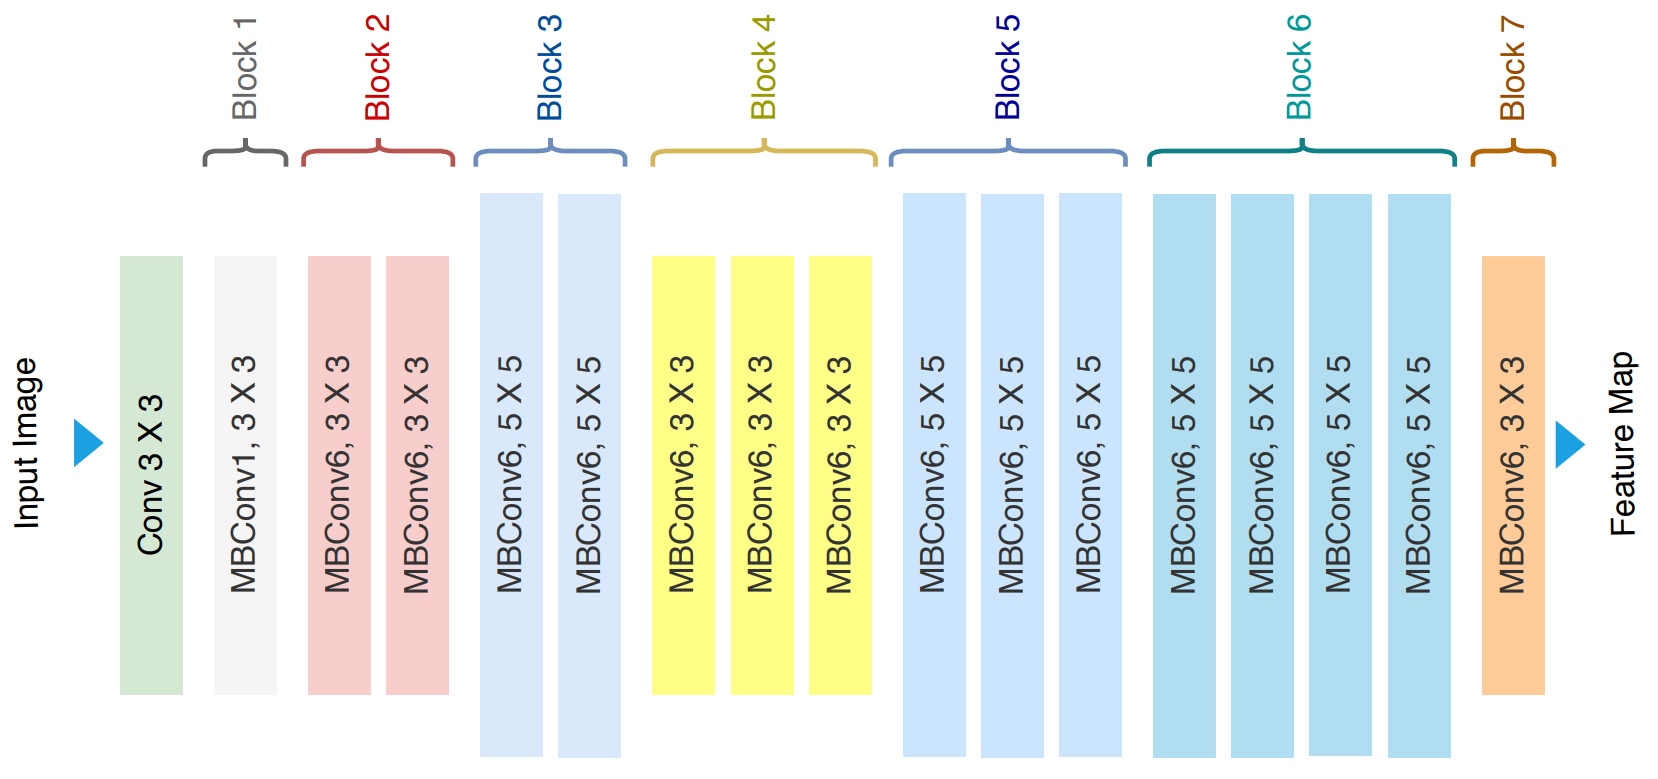
\includegraphics[width=0.95\textwidth]{Figuras/efficientnet.png}
    \caption[Arquitectura de la red EfficientNet.]{Arquitectura de la red EfficientNet. Fuente: \cite{ahmed2021}.}
    \label{fig:efficientnet}
\end{figure}

Inicialmente, esta red se entrenó usando el conjunto de datos ImageNet, donde obtuvo una precisión de 0.933 (el artículo no especifica el F1 score alcanzado) \cite{tan-2019} en la tarea de reconocimiento de objetos en imágenes. Adicionalmente, el artículo destaca que esta precisión es alcanzada entre 5.7 y 6.1 veces más rápido que otras arquitecturas, como ResNet.

En \cite{bjerge-2023}, se utilizó esta red con un conjunto de datos de 1622 imágenes de insectos. Estas imágenes fueron tomadas de \cite{XIE2015123}, donde se tenían 24 especies diferentes de insectos (algunos ejemplos pueden verse en la Figura \ref{fig:efficientnet-insects}). Se obtuvo una precisión de entre 0.9095 y 0.9751 (dependiendo de la cantidad de clases utilizadas).

\begin{figure}[ht]
    \centering
    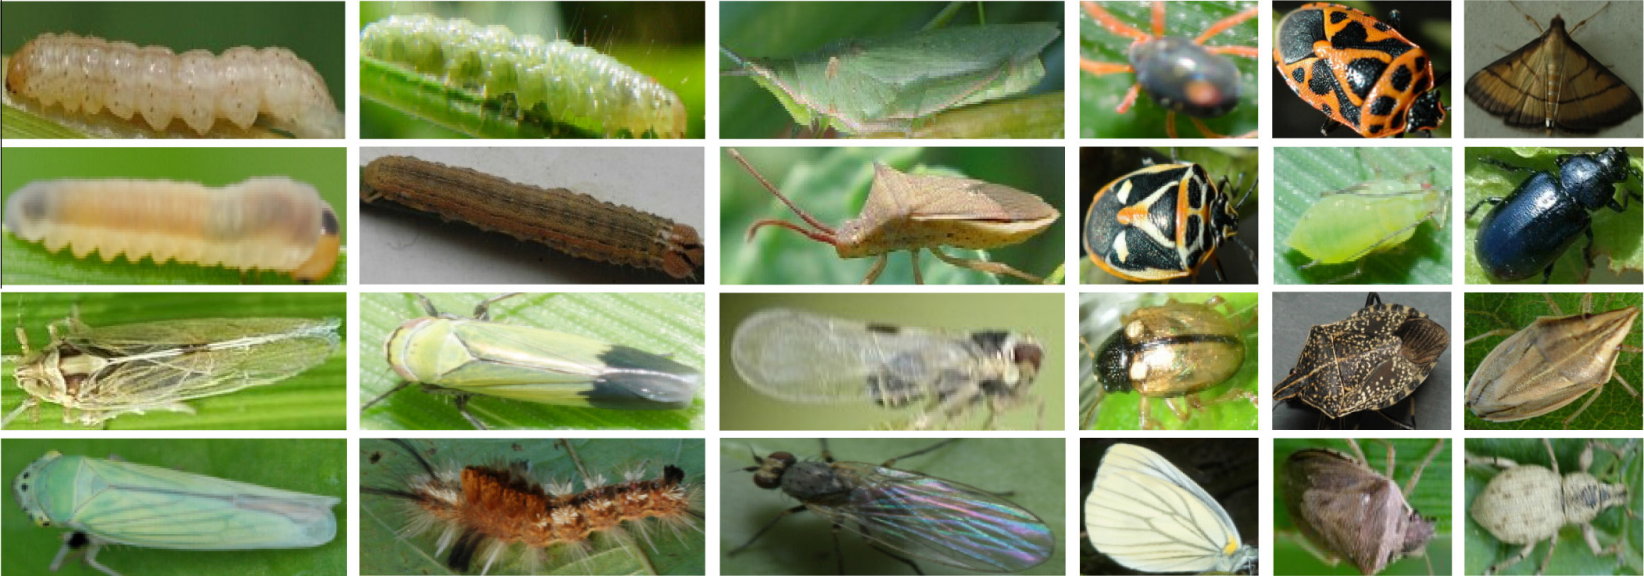
\includegraphics[width=0.95\textwidth]{Figuras/efficientnet-insects.png}
    \caption[Ejemplos de imágenes de insectos utilizadas en {[20]}.]{Ejemplos de imágenes de insectos utilizadas en \cite{bjerge-2023}. Fuente: \cite{bjerge-2023}.}
    \label{fig:efficientnet-insects}
\end{figure}

\subsection{Otras arquitecturas}

Cabe indicar que, YOLOv5 y EfficientNet no son las únicas arquitecturas que han sido sometidas a conjuntos específicos de insectos. En \cite{li-2021} se cuenta con un análisis detallado de modelos usados en la detección de insectos en imágenes. En la Tabla \ref{table:arquitecturas} se presenta un resumen de los resultados obtenidos con los modelos más relevantes.

\begin{table}[H]

\centering\small
\begin{tabular}{@{}lrrr@{}}
\toprule
    \textbf{Modelo} & \textbf{Imágenes} & \textbf{Categorías} & \textbf{Precisión}
\\ \midrule
    Small-sample learning \cite{yang-2021}& 11000 & 220 & 0.5765\\
    Tiny YOLOv3 \cite{rustia-2021} & 400 & 5 & 0.9800\\
    Fine-tuned ResNet-50 \cite{malathi-2021}& 3549 & 10 & 0.9501\\
    Ensemble CNNs \cite{khanramaki-2021}& 1774 & 3 & 0.9904\\
    EfficientNet-B6 \cite{sagar-2020} & 170000 & 1300 & 0.8650\\
    GoogLeNet \cite{li-2020} & 5629 & 10 & 0.9461\\
    ResNet-101 \cite{cheng-2017}& 550 & 10 & 0.9867\\
    AlexNet \cite{liu-2016}& 5000 & 12 & 0.9510\\
\bottomrule
\end{tabular}
\caption[Arquitecturas utilizadas en la detección de insectos en imágenes.]{Resumen de arquitecturas utilizadas en la detección de insectos en imágenes. Fuente \cite{li-2021}.}
\label{table:arquitecturas}
\end{table}

\subsection{Posibles dificultades}

Li, et al. \cite{li-2021} indican que, a pesar de que los modelos de detección de objetos en imágenes presenta buenos resultados, en el caso de realizar reconocimiento de insectos sobre plantas, se pueden presentar algunas dificultades. Las más relevantes para este trabajo son: la complejidad del fondo de la imagen, los diversos tamaños de los insectos y el desbalance de clases. Con respecto a los dos primeros problemas, se tiene que arquitecturas de la familia YOLO presentan buenos resultados en este aspecto \cite{he-2020}.

Para solventar el desbalance de clases, se aplicarán técnicas de aumento de datos (\textit{data augmentation}), las mismas que serán descritas en la siguiente sección.

\section{Preprocesamiento de imágenes}

Dado un conjunto de imágenes, el primer paso es realizar un preprocesamiento de las mismas antes de ser utilizadas en un modelo. Este preprocesamiento va desde el etiquetado hasta el aumento de datos.

A pesar de los múltiples conjuntos de datos sobre insectos (ver \cite{li-2021}, Tabla~3), en este trabajo se usará un conjunto de datos propio. Por lo tanto, se debe realizar el etiquetado de las imágenes; para esto, existen herramientas como \textit{LabelImg} \cite{LabelImg}, orientadas tanto al etiquetado de objetos como a su localización.

Posteriormente, se debe realizar una redimensión de las imágenes, de tal manera que todas tengan el mismo tamaño. Esto es necesario para que el modelo pueda procesar las imágenes de manera eficiente. A continuación, para solventar problemas de limitación de variedad de clases y localizaciones, se puede realizar un aumento de datos, el cual consiste en generar nuevas imágenes a partir de las imágenes originales. Para esto, se pueden utilizar técnicas como el volteo horizontal y vertical, el recorte de imágenes, el cambio de brillo, entre otras. Adicionalmente, al tratarse de imágenes de insectos, es usual que no se tenga un enfoque apropiado en el objetivo, para solventar esto, a partir de imágenes con enfoque adecuado, se puede agregar ruido Gaussiano para simular el desenfoque \cite{khanramaki-2021}.


\section{Redes de polinización}

Las redes de polinización son redes de interacción entre especies de plantas y polinizadores. Contar con este tipo de redes de un determinado ecosistema es esencial para entender la dinámica de las interacciones entre las especies, lo cual es importante para la estabilidad de los ecosistemas y, por ende, para la conservación de la biodiversidad.

Estas redes tradicionalmente se construyen mediante observación y trabajo de campo que normalmente son incompletos y, por esto, hace falta aplicar técnicas estadísticas. Para esto, se puede utilizar la metodología propuesta por Young et al. \cite{young-2021}, la cual se resume a continuación.

Se consideran $n_p$ especies de plantas y $n_a$ especies de polinizadores, se tiene la matriz $M = (M_{ij})$, de orden $n_p\times n_a$, donde $M_{ij}$ es el número de veces que se ha detectado una interacción de la especie $j$ con la planta $i$. Se tiene que $M$ podría representar un grafo bipartito ponderado (matriz de incidencia). El objetivo es, a partir de este grafo, generar otro donde se tenga una arista de un polinizador a una planta si el polinizador prefiere a dicha planta; a la representación matricial de este grafo se la denomina $B$. De esta manera, se tiene que $B_{ij}$ es igual a $1$ si la especie $j$ es un polinizador de la planta $i$ y $0$ en caso contrario.

Con esto, Young et al. \cite{young-2021} proponen que $B_{ij}$ representa una variable aleatoria de la cual, al tener la matriz $M$, se puede calcular su probabilidad condicional. Para esto, deducen que
\[
    P(B_{ij}=1|M) = \sum_{B} \int B_{ij} P(B, \theta|M)\, d\theta
\]
donde la suma corre sobre todas las posibles matrices de incidencia y $\theta$ representa todos los parámetros del modelo planteado: cambio al número promedio de visitas ($r$), el efecto del muestreo ($C$) y abundancia de plantas ($\sigma$) e insectos ($\tau$). A pesar de que, con este enfoque, se tiene una distribución de probabilidad para $B$, esta no es computacionalmente efectiva, por lo tanto, se puede utilizar técnicas de Monte Carlo para aproximar la distribución de probabilidad.

Para esto, se tiene que el número de visitas $M_{ij}$ es una variable aleatoria de Poisson con media
\[
    \mu_{ij} = C \sigma_i \tau_j (1 + rB_{ij}).
\]
De esta manera, si se considera que la probabilidad de que un insecto sea polinizador de una planta como una variable uniforme de probabilidad $\rho$, se tiene que
\[
    P(B, \theta|M) \propto P(\theta) \prod_{ij} (1-\rho)^{1-B_{ij}} \rho^{B_{ij}}  \frac{\mu_{ij}^{M_{ij}} }{M_{ij}!}e^{-\mu_{ij}} .
\]
Con esto, se puede utilizar un algoritmo de maximización de la esperanza para obtener los parámetros del modelo y, de esta manera, obtener la distribución de probabilidad de $B$.


Esta metodología proporcionó resultados coherentes con las propiedades de la distribución de conexión que fue propuesta como un invariante en este tipo de redes en \cite{jordano-2002}.